\documentclass{article}

% content/resources/templates/preamble.tex
\usepackage[margin=0.6in]{geometry}
\author{Milav Dabgar}
\usepackage{amsmath,amssymb,amsthm}
\usepackage{booktabs}
\usepackage{multirow}
\usepackage{xcolor}
\usepackage{tcolorbox}
\tcbuselibrary{breakable,skins}
\usepackage[colorlinks=true,linkcolor=blue]{hyperref}
\usepackage{titlesec}
\usepackage{enumitem}
\usepackage{tikz}
\usepackage{pgfplots}
\usepackage{circuitikz}
\usepackage[version=4]{mhchem}
\usepackage{longtable}
\usepackage{array}
\usepackage{float}
\usepackage{caption}
\usepackage{listings}

\lstset{
  basicstyle=\small\ttfamily,
  breaklines=true,
  breakatwhitespace=false,
  postbreak=\mbox{\textcolor{red}{$\hookrightarrow$}\space},
  float=false,
  numbers=left,
  numberstyle=\tiny\color{gray},
  numbersep=10pt,
  xleftmargin=2em,
  keywordstyle=\color{blue},
  commentstyle=\color{green!60!black},
  stringstyle=\color{purple},
  backgroundcolor=\color{gray!5},
  showstringspaces=false,
  tabsize=2,
  captionpos=b,
  keepspaces=true,
  columns=flexible
}

\pgfplotsset{compat=1.18}
\usetikzlibrary{shapes,arrows,positioning,calc,patterns,decorations.pathmorphing,decorations.markings,arrows.meta}

% Color scheme
\definecolor{headcolor}{RGB}{0,102,204}
\definecolor{keycolor}{RGB}{220,20,60}
\definecolor{solutioncolor}{RGB}{34,139,34}
\definecolor{mnemoniccolor}{RGB}{148,0,211}
\definecolor{codecolor}{RGB}{0,0,100}

% Spacing
\setlength{\parskip}{3pt}
\setlist[itemize]{nosep}
\setlist[enumerate]{nosep}

% Title formatting
\titleformat{\section}{\Large\bfseries\color{headcolor}}{\thesection}{1em}{}
\titleformat{\subsection}{\large\bfseries\color{headcolor}}{\thesubsection}{1em}{}

% Pandoc tightlist compatibility
\providecommand{\tightlist}{%
  \setlength{\itemsep}{0pt}\setlength{\parskip}{0pt}}

% Pandoc longtable compatibility
\newcounter{none}
\def\thenone{}


% content/resources/templates/english-boxes.tex

% Custom environments
\newtcolorbox{solutionbox}{
 breakable,
 enhanced,
 colback=solutioncolor!5!white,
 colframe=solutioncolor!75!black,
 fonttitle=\bfseries,
 title=Solution
}

\newtcolorbox{solutionboxnobreak}{
 colback=solutioncolor!5!white,
 colframe=solutioncolor!75!black,
 fonttitle=\bfseries,
 title=Solution
}

\newtcolorbox{keyformula}{
 breakable,
 enhanced,
 colback=keycolor!5!white,
 colframe=keycolor!75!black,
 fonttitle=\bfseries,
 title=Key Formula
}

\newtcolorbox{mnemonicboxenv}{
 breakable,
 enhanced,
 colback=mnemoniccolor!5!white,
 colframe=mnemoniccolor!75!black,
 fonttitle=\bfseries,
 title=Mnemonic
}

\newcommand{\mnemonicbox}[1]{%
  \begin{mnemonicboxenv}
    #1
  \end{mnemonicboxenv}
}


% Custom commands for GTU solutions
% This file defines semantic commands for consistent formatting

% Question command with automatic formatting
\newcommand{\question}[2]{%
  \section*{Question #1}%
  \textbf{#2}%
}

% OR question variant
\newcommand{\questionor}[2]{%
  \section*{Question #1 OR}%
  \textbf{#2}%
}

% Proper table environment with caption
\newenvironment{answertable}[1]{%
  \begin{table}[htbp]
  \centering
  \caption{#1}
}{%
  \end{table}
}

% Proper figure environment for diagrams
\newenvironment{answerdiagram}[1]{%
  \begin{figure}[htbp]
  \centering
  \caption{#1}
}{%
  \end{figure}
}

% Semantic markup for key terms
\newcommand{\keyword}[1]{\textbf{#1}}
\newcommand{\code}[1]{\texttt{#1}}
\newcommand{\classname}[1]{\texttt{#1}}
\newcommand{\methodname}[1]{\texttt{#1}}

% Proper quotation marks
\newcommand{\mnemonic}[1]{``#1''}

\usetikzlibrary{matrix}

\title{Microprocessor and Microcontroller (4341101) - Summer 2023 Solution}
\date{June 15, 2023}

\begin{document}
\maketitle

\questionmarks{1}{a}{3}
\textbf{Compare Microprocessor and Microcontroller.}

\begin{solutionbox}
\textbf{Answer}:

\begin{center}
\captionof{table}{Microprocessor vs Microcontroller}
\begin{tabular}{|l|p{5cm}|p{5cm}|}
\hline
\textbf{Feature} & \textbf{Microprocessor} & \textbf{Microcontroller} \\ \hline
Definition & CPU on single chip & Complete computer on single chip \\ \hline
Memory & External RAM/ROM needed & Built-in RAM/ROM \\ \hline
Applications & General computing, PCs & Embedded systems, IoT \\ \hline
Examples & Intel 8085, 8086 & 8051, Arduino, PIC \\ \hline
Cost & Higher & Lower \\ \hline
\end{tabular}
\end{center}
\end{solutionbox}
\begin{mnemonicbox}
``PCRAM'' - ``Processors Connect to RAM, Microcontrollers Already have Memory''
\end{mnemonicbox}

\questionmarks{1}{b}{4}
\textbf{Compare RISC and CISC.}

\begin{solutionbox}
\textbf{Answer}:

\begin{center}
\captionof{table}{RISC vs CISC}
\begin{tabular}{|l|p{6cm}|p{6cm}|}
\hline
\textbf{Feature} & \textbf{RISC (Reduced Instruction Set Computer)} & \textbf{CISC (Complex Instruction Set Computer)} \\ \hline
Instructions & Few, simple instructions & Many, complex instructions \\ \hline
Execution Time & Fixed (1 clock cycle) & Variable (multiple cycles) \\ \hline
Memory Access & Only through load/store & Multiple memory access modes \\ \hline
Pipelining & Easy implementation & Difficult implementation \\ \hline
Examples & ARM, MIPS & Intel x86, 8085 \\ \hline
Hardware & Simple, less transistors & Complex, more transistors \\ \hline
Register Set & Large number of registers & Fewer registers \\ \hline
\end{tabular}
\end{center}
\end{solutionbox}
\begin{mnemonicbox}
``RISC-Fast, CISC-Many'' (RISC uses Fast execution, CISC has Many instructions)
\end{mnemonicbox}

\questionmarks{1}{c}{7}
\textbf{Define: Microprocessor, Operand, Instruction Cycle, Opcode, ALU, Machine Cycle, T-State}

\begin{solutionbox}
\textbf{Answer}:

\begin{center}
\captionof{table}{Definitions}
\begin{tabular}{|l|p{10cm}|}
\hline
\textbf{Term} & \textbf{Definition} \\ \hline
\textbf{Microprocessor} & CPU on a single integrated circuit that processes instructions \\ \hline
\textbf{Operand} & Data value used in an instruction operation \\ \hline
\textbf{Instruction Cycle} & Complete process to fetch, decode and execute an instruction \\ \hline
\textbf{Opcode} & Operation code that tells CPU what operation to perform \\ \hline
\textbf{ALU} & Arithmetic Logic Unit that performs mathematical computations \\ \hline
\textbf{Machine Cycle} & Basic operation like memory read/write (subset of instruction cycle) \\ \hline
\textbf{T-State} & Time state - smallest unit of time in processor operation (clock period) \\ \hline
\end{tabular}
\end{center}

\begin{center}
\begin{tikzpicture}[node distance=2.5cm, auto]
    \node [gtu block] (fetch) {FETCH\\Get instruction\\from memory};
    \node [gtu block, right of=fetch] (decode) {DECODE\\Interpret opcode\\Identify operands};
    \node [gtu block, right of=decode] (execute) {EXECUTE\\Perform operation\\Store results};
    
    \draw [gtu arrow] (fetch) -- (decode);
    \draw [gtu arrow] (decode) -- (execute);
    \draw [gtu arrow] (execute) -- ++(0,-1.5) -| (fetch);
    
    \node [below of=decode, node distance=1.8cm] {INSTRUCTION CYCLE};
\end{tikzpicture}
\end{center}
\end{solutionbox}
\begin{mnemonicbox}
``My Old Intel Chip Only Makes Trouble'' (Microprocessor, Operand, Instruction, Opcode, ALU, Machine, T-state)
\end{mnemonicbox}

\orquestionmarks{1}{c}{7}
\textbf{Compare Von-Neumann and Harvard architecture.}

\begin{solutionbox}
\textbf{Answer}:

\begin{center}
\captionof{table}{Von-Neumann vs Harvard Architecture}
\begin{tabular}{|l|p{6cm}|p{6cm}|}
\hline
\textbf{Feature} & \textbf{Von-Neumann Architecture} & \textbf{Harvard Architecture} \\ \hline
Memory Buses & Single memory bus for instructions and data & Separate buses for program and data memory \\ \hline
Execution & Sequential execution & Parallel fetch and execute possible \\ \hline
Speed & Slower due to bus bottleneck & Faster due to simultaneous access \\ \hline
Complexity & Simpler design & More complex design \\ \hline
Applications & General-purpose computing & DSP, microcontrollers, embedded systems \\ \hline
Security & Less secure (code can be modified as data) & More secure (code separation from data) \\ \hline
Example & Most PCs, 8085, 8086 & 8051, PIC, ARM Cortex-M \\ \hline
\end{tabular}
\end{center}

\begin{center}
\begin{tikzpicture}[node distance=2cm]
    % Von Neumann
    \node (v_cpu) [gtu block] {CPU};
    \node (v_mem) [gtu block, right of=v_cpu, node distance=3cm] {Memory\\(Code + Data)};
    \draw [gtu arrow, <->] (v_cpu) -- node[above] {Bus} (v_mem);
    \node [below of=v_cpu, node distance=1.5cm] {Von-Neumann};

    % Harvard
    \node (h_cpu) [gtu block, right of=v_mem, node distance=4cm] {CPU};
    \node (h_prog) [gtu block, right of=h_cpu, node distance=3cm, yshift=1cm] {Program\\Memory};
    \node (h_data) [gtu block, right of=h_cpu, node distance=3cm, yshift=-1cm] {Data\\Memory};
    \draw [gtu arrow, <->] (h_cpu) -- (h_prog);
    \draw [gtu arrow, <->] (h_cpu) -- (h_data);
    \node [below of=h_cpu, node distance=1.5cm] {Harvard};
\end{tikzpicture}
\end{center}
\end{solutionbox}
\begin{mnemonicbox}
``Harvard Has Separate Streets'' (Harvard Has Separate memory paths)
\end{mnemonicbox}

\questionmarks{2}{a}{3}
\textbf{Draw Flag Register of 8085 microprocessor \& explain it.}

\begin{solutionbox}
\textbf{Answer}:

\begin{center}
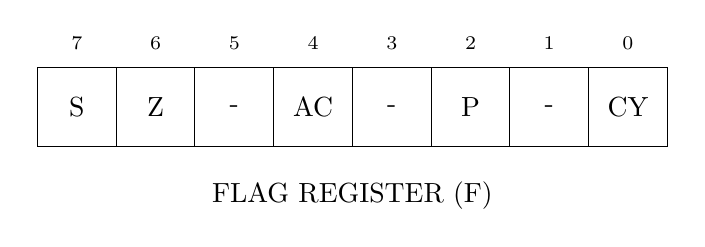
\begin{tikzpicture}
    % Flag Register
    \matrix (flags) [matrix of nodes, nodes={draw, minimum size=1cm, anchor=center}, column sep=-\pgflinewidth] {
        S & Z & - & AC & - & P & - & CY \\
    };
    
    % Bit numbers
    \foreach \i [count=\xi from 1] in {7,6,5,4,3,2,1,0} {
        \node [above=0.1cm of flags-1-\xi, font=\scriptsize] {\i};
    }
    
    \node [below=0.2cm of flags] {FLAG REGISTER (F)};
\end{tikzpicture}
\end{center}

\begin{center}
\captionof{table}{Flag Register Bits}
\begin{tabular}{|l|l|l|}
\hline
\textbf{Flag} & \textbf{Name} & \textbf{Purpose} \\ \hline
S & Sign & Set if result is negative (bit 7=1) \\ \hline
Z & Zero & Set if result is zero \\ \hline
AC & Auxiliary Carry & Set if carry from bit 3 to bit 4 \\ \hline
P & Parity & Set if result has even parity \\ \hline
CY & Carry & Set if carry from bit 7 or borrow to bit 7 \\ \hline
\end{tabular}
\end{center}
\end{solutionbox}
\begin{mnemonicbox}
``Smart Zombies Always Prefer Candy'' (Sign, Zero, Auxiliary, Parity, Carry)
\end{mnemonicbox}

\questionmarks{2}{b}{4}
\textbf{Explain De-multiplexing of Address and Data buses for 8085 Microprocessor.}

\begin{solutionbox}
\textbf{Answer}:

\begin{center}
\begin{tikzpicture}[auto, node distance=2.5cm]
    \node [gtu block, minimum width=3cm, minimum height=4cm] (cpu) {8085 CPU};
    \node [gtu block, right of=cpu, node distance=5cm, yshift=-1.5cm] (latch) {74LS373\\Latch};
    
    % Higher Order Address
    \draw [->, thick] (cpu.north east) ++(0,-0.5) -- ++(2,0) node[right] {A15-A8 (Higher Address)};
    
    % Address/Data Bus
    \draw [thick] (cpu.east) ++(0,-1.5) -- ++(1.5,0) coordinate (split);
    \draw [thick] (split) -- (latch.west) node[midway, above] {AD7-AD0};
    \draw [<->, thick] (split) -- ++(0, -1.5) node[below] {Data Bus D7-D0};
    
    % ALE
    \draw [->] (cpu.east) ++(0,-2.5) -- ++(1.5,0) -- (latch.south) node[midway, right] {ALE};
    
    % Latch output
    \draw [->, thick] (latch.east) -- ++(1.5,0) node[right] {A7-A0 (Lower Address)};
    
    % Labels
    \node at (cpu.east) [yshift=-1.5cm, xshift=-1cm] {AD7-AD0};
    \node at (cpu.east) [yshift=-2.5cm, xshift=-1cm] {ALE};
    \node at (cpu.east) [yshift=-0.5cm, xshift=-1cm] {A15-A8};

\end{tikzpicture}
\end{center}

\begin{itemize}
    \item \textbf{Need}: 8085 has multiplexed pins (AD0-AD7) to save pins
    \item \textbf{Process}:
    \begin{enumerate}
        \item CPU places address on AD0-AD7 pins
        \item ALE (Address Latch Enable) signal goes HIGH
        \item Address latch (74LS373) captures lower address bits
        \item ALE goes LOW, latching the address
        \item AD0-AD7 pins now free for data transfer
    \end{enumerate}
\end{itemize}
\end{solutionbox}
\begin{mnemonicbox}
``ALE Latches, Data Follows'' (Address Latch Enable captures address first, then data)
\end{mnemonicbox}

\questionmarks{2}{c}{7}
\textbf{Describe architecture of 8085 microprocessor with the help of neat diagram.}

\begin{solutionbox}
\textbf{Answer}:

\begin{center}
\begin{tikzpicture}[node distance=2cm]
    % Outer block as CPU
    \node [draw, rectangle, minimum width=8cm, minimum height=6cm, fill=black!5, rounded corners] (cpu) {};
    \node [below right] at (cpu.north west) {\textbf{8085 CPU}};

    % Internal components
    \node [gtu block, fill=white] (regs) at ([xshift=-2cm, yshift=1.5cm]cpu.center) {REGISTERS\\A, B, C, D\\E, H, L\\SP, PC};
    \node [gtu block, fill=white, right of=regs, node distance=4cm] (control) {CONTROL UNIT\\Timing \&\\Control};
    \node [gtu block, fill=white, below of=regs, node distance=3cm] (alu) {ALU};
    
    % Connections
    \draw [gtu arrow, <->] (regs) -- (alu);
    \draw [gtu arrow] (control) -- (regs);
    \draw [gtu arrow] (control) -- (alu);
    
    % Buses
    \node [gtu block, fill=white] (bus) at ([yshift=-2.5cm]cpu.center) {Address/Data Buffers};
    \draw [gtu arrow, <->] (alu) -- (bus);
    \draw [gtu arrow, <->] (regs) -- (bus);
    
    % External connections
    \draw [gtu arrow] (bus.south) -- ++(0,-1) node[below] {Address \& Data Bus};
    \draw [gtu arrow] (control.east) -- ++(1,0) node[right] {Control Signals};

\end{tikzpicture}
\end{center}

\begin{itemize}
    \item \textbf{Main Components}:
    \begin{itemize}
        \item \textbf{Registers}: Storage locations (A, B-L, SP, PC, Flags)
        \item \textbf{ALU}: Performs arithmetic and logical operations
        \item \textbf{Control Unit}: Generates timing and control signals
        \item \textbf{Buses}: Address bus (16-bit), Data bus (8-bit), Control bus
    \end{itemize}
    \item \textbf{Key Features}:
    \begin{itemize}
        \item 8-bit data bus, 16-bit address bus (64KB addressable memory)
        \item 6 general-purpose registers (B,C,D,E,H,L) and accumulator
        \item 5 flags for status information
    \end{itemize}
\end{itemize}
\end{solutionbox}
\begin{mnemonicbox}
``RABC'' - ``Registers, ALU, Buses, Control'' (main components)
\end{mnemonicbox}

\orquestionmarks{2}{a}{3}
\textbf{Explain Bus Organization of 8085 microprocessor.}

\begin{solutionbox}
\textbf{Answer}:

\begin{center}
\captionof{table}{8085 Bus Organization}
\begin{tabular}{|l|l|l|}
\hline
\textbf{Bus Type} & \textbf{Width} & \textbf{Function} \\ \hline
\textbf{Address Bus} & 16-bit (A0-A15) & Carries memory/I/O device addresses \\ \hline
\textbf{Data Bus} & 8-bit (D0-D7) & Transfers data between CPU \& memory/I/O \\ \hline
\textbf{Control Bus} & Various signals & Coordinates system operations \\ \hline
\end{tabular}
\end{center}

\textbf{Key Control Signals}:
\begin{itemize}
    \item \textbf{$\overline{RD}$}: Read signal (active low)
    \item \textbf{$\overline{WR}$}: Write signal (active low)
    \item \textbf{ALE}: Address Latch Enable
    \item \textbf{$IO/\overline{M}$}: Distinguishes I/O (high) from memory (low) operations
\end{itemize}

\begin{center}
\begin{tikzpicture}[node distance=2cm, auto]
    \node [gtu block] (cpu) {8085 CPU};
    
    \draw [->, thick] (cpu.south) ++(-1.5,0) -- ++(0,-1.5) node[below, align=center] {Address Bus\\(16-bit)};
    \draw [<->, thick] (cpu.south) -- ++(0,-1.5) node[below, align=center] {Data Bus\\(8-bit)};
    \draw [->, thick] (cpu.south) ++(1.5,0) -- ++(0,-1.5) node[below, align=center] {Control Bus\\(RD, WR, etc.)};
\end{tikzpicture}
\end{center}
\end{solutionbox}
\begin{mnemonicbox}
``ADC'' - ``Address finds, Data travels, Control coordinates''
\end{mnemonicbox}

\orquestionmarks{2}{b}{4}
\textbf{Explain: Program Counter \& Stack pointer}

\begin{solutionbox}
\textbf{Answer}:

\begin{center}
\captionof{table}{PC vs SP}
\begin{tabular}{|l|l|p{6cm}|}
\hline
\textbf{Register} & \textbf{Size} & \textbf{Function} \\ \hline
\textbf{Program Counter (PC)} & 16-bit & Holds address of next instruction to execute \\ \hline
\textbf{Stack Pointer (SP)} & 16-bit & Points to the top of the stack in memory \\ \hline
\end{tabular}
\end{center}

\textbf{Program Counter (PC)}:
\begin{itemize}
    \item Automatically increments after instruction fetch
    \item Modified by jump/call instructions
    \item Controls program execution sequence
    \item Initially set to 0000H on reset
\end{itemize}

\textbf{Stack Pointer (SP)}:
\begin{itemize}
    \item Points to last data item pushed onto stack
    \item Stack works in LIFO (Last In First Out) manner
    \item Used during subroutine calls and interrupts
    \item Stack grows downward in memory (decrements)
\end{itemize}

\begin{center}
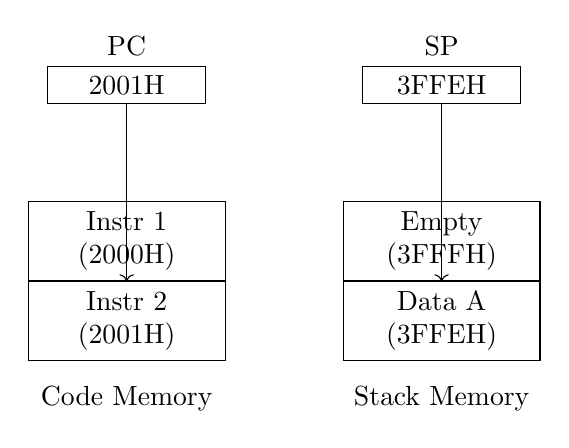
\begin{tikzpicture}
    % PC
    \node [draw, rectangle, minimum width=2cm, label=above:PC] (pc) at (0,3) {2001H};
    
    % SP
    \node [draw, rectangle, minimum width=2cm, label=above:SP] (sp) at (4,3) {3FFEH};
    
    % Code Memory
    \node [draw, rectangle, minimum width=2.5cm, minimum height=1cm, align=center] (code2) at (0,0) {Instr 2\\(2001H)};
    \node [draw, rectangle, minimum width=2.5cm, minimum height=1cm, align=center, above=0cm of code2] (code1) {Instr 1\\(2000H)};
    \draw [->] (pc) -- (code2);
    
    % Stack Mem
    \node [draw, rectangle, minimum width=2.5cm, minimum height=1cm, align=center] (stack1) at (4,0) {Data A\\(3FFEH)};
    \node [draw, rectangle, minimum width=2.5cm, minimum height=1cm, align=center, above=0cm of stack1] (stack0) {Empty\\(3FFFH)};
    \draw [->] (sp) -- (stack1);
    
    \node [below=0.2cm of code2] {Code Memory};
    \node [below=0.2cm of stack1] {Stack Memory};

\end{tikzpicture}
\end{center}
\end{solutionbox}
\begin{mnemonicbox}
``PC Previews, SP Stacks'' (PC points to next instruction, SP manages stack)
\end{mnemonicbox}

\orquestionmarks{2}{c}{7}
\textbf{Describe Pin diagram of 8085 microprocessor with the help of neat diagram.}

\begin{solutionbox}
\textbf{Answer}:

\begin{center}
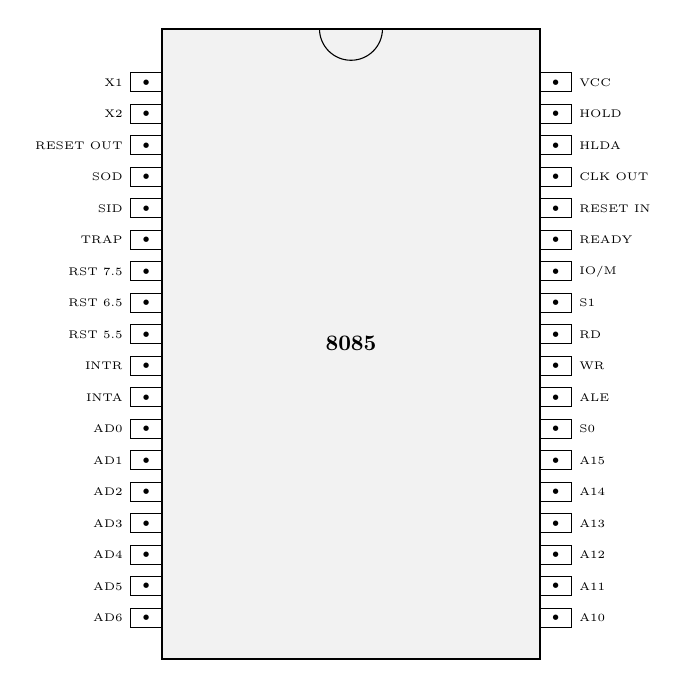
\begin{tikzpicture}[scale=0.8, transform shape]
    % Chip Body
    \draw[thick, fill=gray!10] (0,0) rectangle (6,10);
    \node at (3,5) {\textbf{8085}};
    \draw (2.5,10) arc (180:360:0.5); % Notch

    % Pins Left
    \foreach \name/\y in {X1/9, X2/8.5, RESET OUT/8, SOD/7.5, SID/7, TRAP/6.5, RST 7.5/6, RST 6.5/5.5, RST 5.5/5, INTR/4.5, INTA/4, AD0/3.5, AD1/3, AD2/2.5, AD3/2, AD4/1.5, AD5/1, AD6/0.5} {
        \draw (-0.5,\y) rectangle (0,\y+0.3);
        \node[left, font=\tiny] at (-0.5,\y+0.15) {\name};
        \node[font=\tiny] at (-0.25,\y+0.15) {\tiny $\bullet$};
    }
    
    % Pins Right
    \foreach \name/\y in {VCC/9, HOLD/8.5, HLDA/8, CLK OUT/7.5, RESET IN/7, READY/6.5, {IO/M}/6, S1/5.5, RD/5, WR/4.5, ALE/4, S0/3.5, A15/3, A14/2.5, A13/2, A12/1.5, A11/1, A10/0.5} {
        \draw (6,\y) rectangle (6.5,\y+0.3);
        \node[right, font=\tiny] at (6.5,\y+0.15) {\name};
        \node[font=\tiny] at (6.25,\y+0.15) {\tiny $\bullet$};
    }
    
\end{tikzpicture}
\end{center}

\textbf{Pin Groups}:
\begin{enumerate}
    \item \textbf{Power \& Clock}: Vcc, GND, X1, X2, CLK
    \item \textbf{Address/Data}: A8-A15, AD0-AD7 (multiplexed)
    \item \textbf{Control}: ALE, $\overline{RD}$, $\overline{WR}$, $IO/\overline{M}$
    \item \textbf{Interrupt}: INTR, $\overline{INTA}$, RST 5.5/6.5/7.5, TRAP
    \item \textbf{DMA}: HOLD, HLDA
    \item \textbf{Serial I/O}: SID, SOD
    \item \textbf{Status}: S0, S1
\end{enumerate}
\end{solutionbox}
\begin{mnemonicbox}
``PACI-DHS'' (Power, Address, Control, Interrupt, DMA, Hardware status, Serial)
\end{mnemonicbox}

\questionmarks{3}{a}{3}
\textbf{Explain Stack, Stack Pointer and Stack operation.}

\begin{solutionbox}
\textbf{Answer}:

\begin{center}
\captionof{table}{Stack Concepts}
\begin{tabular}{|l|p{10cm}|}
\hline
\textbf{Term} & \textbf{Definition} \\ \hline
\textbf{Stack} & Memory area used for temporary storage in LIFO order \\ \hline
\textbf{Stack Pointer} & 16-bit register that points to the top item in stack \\ \hline
\textbf{PUSH} & Operation that stores data on stack (SP decrements) \\ \hline
\textbf{POP} & Operation that retrieves data from stack (SP increments) \\ \hline
\end{tabular}
\end{center}

\begin{center}
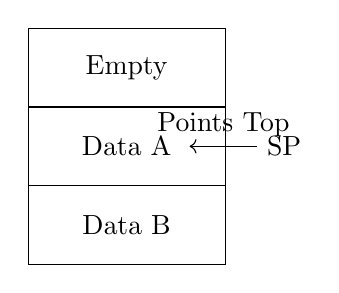
\begin{tikzpicture}[node distance=1.5cm]
    % Stack Mem
    \node [draw, rectangle, minimum width=2.5cm, minimum height=3cm, fill=white] (stack) at (0,0) {};
    \draw (-1.25, 0.5) -- (1.25, 0.5);
    \draw (-1.25, -0.5) -- (1.25, -0.5);
    \node at (0, 1) {Empty};
    \node at (0, 0) {Data A};
    \node at (0, -1) {Data B};
    
    \node [right of=stack, node distance=2cm] (sp) {SP};
    \draw [->] (sp) -- (0.8, 0) node [midway, above] {Points Top};
\end{tikzpicture}
\end{center}
\end{solutionbox}
\begin{mnemonicbox}
``LIFO Saves Push-Pop'' (Last-In-First-Out with Push and Pop operations)
\end{mnemonicbox}

\questionmarks{3}{b}{4}
\textbf{Draw Timers/Counters logic diagram of 8051 microcontroller and explain it.}

\begin{solutionbox}
\textbf{Answer}:

\begin{center}
\begin{tikzpicture}[auto, node distance=2cm]
    \node [gtu block] (control) {Control Logic\\(TMOD, TCON)};
    \node [gtu block, right of=control, node distance=4cm] (timer) {Timer Register\\(THx, TLx)};
    \node [right of=timer, node distance=3cm, align=center] (flag) {Overflow Flag\\(TFx)};
    
    \draw [->] (control) -- (timer);
    \draw [->] (timer) -- (flag);
    
    \node [left of=control, node distance=3cm] (osc) {Oscillator / 12};
    \node [below of=osc, node distance=1.5cm] (pin) {Ext. Pin (Tx)};
    
    \draw [->] (osc) -- node {Timer Mode} (control);
    \draw [->] (pin) -- node [swap] {Counter Mode} (control);

\end{tikzpicture}
\end{center}

\begin{itemize}
    \item \textbf{8051 has 2 16-bit timers/counters}: Timer 0 and Timer 1
    \item \textbf{Each timer has two 8-bit registers}: THx (High byte) and TLx (Low byte)
    \item \textbf{4 Operating Modes}:
    \begin{itemize}
        \item Mode 0: 13-bit timer
        \item Mode 1: 16-bit timer
        \item Mode 2: 8-bit auto-reload
        \item Mode 3: Split timer mode
    \end{itemize}
    \item \textbf{Two Functions}:
    \begin{itemize}
        \item Timer: Counts internal clock pulses
        \item Counter: Counts external events
    \end{itemize}
\end{itemize}
\end{solutionbox}
\begin{mnemonicbox}
``TIME-C'' (Timer Input, Mode select, External count)
\end{mnemonicbox}

\questionmarks{3}{c}{7}
\textbf{With the help of neat diagram explain Pin diagram of 8051 microcontroller.}

\begin{solutionbox}
\textbf{Answer}:

\begin{center}
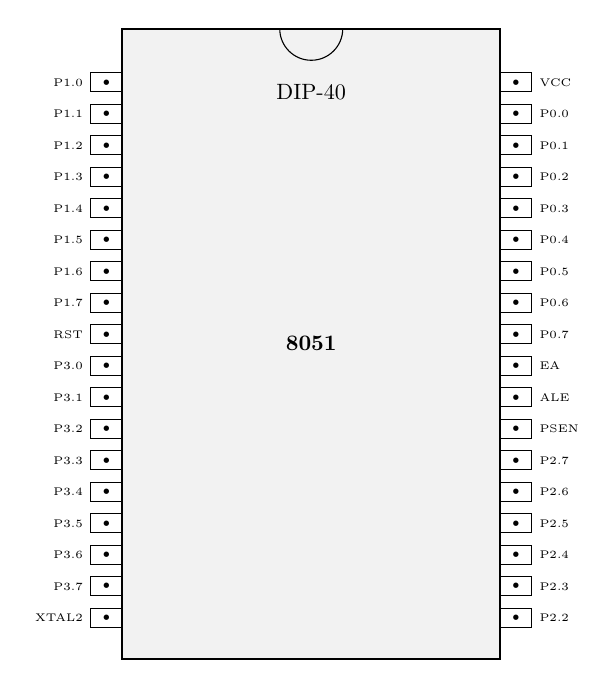
\begin{tikzpicture}[scale=0.8, transform shape]
    % Chip Body
    \draw[thick, fill=gray!10] (0,0) rectangle (6,10);
    \node at (3,5) {\textbf{8051}};
    \node at (3,9) {DIP-40};
    \draw (2.5,10) arc (180:360:0.5); % Notch

    % Pins Left
    \foreach \name/\y in {P1.0/9, P1.1/8.5, P1.2/8, P1.3/7.5, P1.4/7, P1.5/6.5, P1.6/6, P1.7/5.5, RST/5, P3.0/4.5, P3.1/4, P3.2/3.5, P3.3/3, P3.4/2.5, P3.5/2, P3.6/1.5, P3.7/1, XTAL2/0.5} {
        \draw (-0.5,\y) rectangle (0,\y+0.3);
        \node[left, font=\tiny] at (-0.5,\y+0.15) {\name};
        \node[font=\tiny] at (-0.25,\y+0.15) {\tiny $\bullet$};
    }
    
    % Pins Right
    \foreach \name/\y in {VCC/9, P0.0/8.5, P0.1/8, P0.2/7.5, P0.3/7, P0.4/6.5, P0.5/6, P0.6/5.5, P0.7/5, EA/4.5, ALE/4, PSEN/3.5, P2.7/3, P2.6/2.5, P2.5/2, P2.4/1.5, P2.3/1, P2.2/0.5} {
        \draw (6,\y) rectangle (6.5,\y+0.3);
        \node[right, font=\tiny] at (6.5,\y+0.15) {\name};
        \node[font=\tiny] at (6.25,\y+0.15) {\tiny $\bullet$};
    }

\end{tikzpicture}
\end{center}

\textbf{Pin Groups}:
\begin{enumerate}
    \item \textbf{Port Pins}:
    \begin{itemize}
        \item P0 (Port 0): 8-bit bidirectional, multiplexed address/data
        \item P1 (Port 1): 8-bit bidirectional I/O
        \item P2 (Port 2): 8-bit bidirectional, higher address byte
        \item P3 (Port 3): 8-bit bidirectional with alternate functions
    \end{itemize}
    \item \textbf{Power \& Clock}: VCC, GND, XTAL1, XTAL2
    \item \textbf{Control Signals}:
    \begin{itemize}
        \item RST: Reset input
        \item ALE: Address Latch Enable
        \item $\overline{PSEN}$: Program Store Enable
        \item $\overline{EA}$: External Access
    \end{itemize}
\end{enumerate}
\end{solutionbox}
\begin{mnemonicbox}
``PORT-CAPS'' (Ports 0-3, Clock, Address latch, Program store, Supply)
\end{mnemonicbox}

\orquestionmarks{3}{a}{3}
\textbf{Explain Serial communication modes of 8051 microcontroller.}

\begin{solutionbox}
\textbf{Answer}:

\begin{center}
\captionof{table}{Serial Modes}
\begin{tabular}{|l|l|l|l|}
\hline
\textbf{Mode} & \textbf{Description} & \textbf{Baud Rate} & \textbf{Data Bits} \\ \hline
\textbf{Mode 0} & Shift register & Fixed ($F_{OSC}/12$) & 8 bits \\ \hline
\textbf{Mode 1} & 8-bit UART & Variable & 10 bits (8+start+stop) \\ \hline
\textbf{Mode 2} & 9-bit UART & Fixed ($F_{OSC}/32$ or $F_{OSC}/64$) & 11 bits (9+start+stop) \\ \hline
\textbf{Mode 3} & 9-bit UART & Variable & 11 bits (9+start+stop) \\ \hline
\end{tabular}
\end{center}

\textbf{Key Components}:
\begin{itemize}
    \item \textbf{SBUF}: Serial buffer register
    \item \textbf{SCON}: Serial control register
    \item \textbf{P3.0 (RXD)}: Receive pin
    \item \textbf{P3.1 (TXD)}: Transmit pin
\end{itemize}

\begin{center}
\begin{tikzpicture}[node distance=2.5cm, auto]
    \node [gtu block] (sbuf) {SBUF};
    \node [gtu block, above of=sbuf, node distance=2cm] (control) {Serial\\Control Logic\\(SCON)};
    \node [gtu block, left of=control, node distance=3.5cm] (baud) {Baud Rate\\Generator\\(Timer 1)};
    \node [right of=control, node distance=3.5cm, align=center] (pins) {TXD (P3.1)\\RXD (P3.0)};
    
    \draw [->] (baud) -- (control);
    \draw [->] (control) -- (sbuf);
    \draw [->] (control) -- (pins);
    \draw [->] (pins) -- (control);
\end{tikzpicture}
\end{center}
\end{solutionbox}
\begin{mnemonicbox}
``SMART'' (Serial Modes Are Rate and Timing dependent)
\end{mnemonicbox}

\orquestionmarks{3}{b}{4}
\textbf{Explain Internal RAM Organization of 8051 microcontroller.}

\begin{solutionbox}
\textbf{Answer}:

\begin{center}
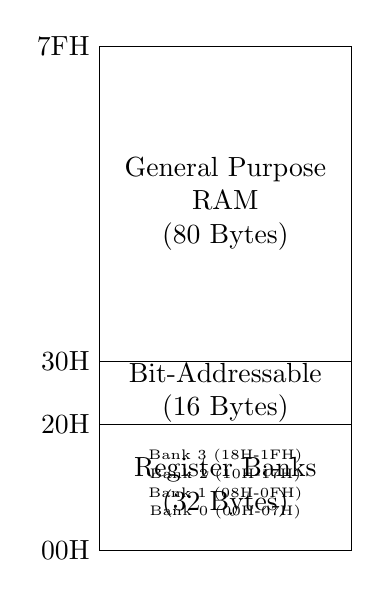
\begin{tikzpicture}[scale=0.8]
    % RAM Block
    \draw (0,0) rectangle (4,8);
    
    % Sections
    \draw (0,2) -- (4,2);
    \draw (0,3) -- (4,3);
    
    % Labels
    \node [align=center] at (2, 5.5) {General Purpose\\RAM\\(80 Bytes)};
    \node [align=center] at (2, 2.5) {Bit-Addressable\\(16 Bytes)};
    \node [align=center] at (2, 1) {Register Banks\\(32 Bytes)};
    
    % Addresses
    \node [left] at (0,8) {7FH};
    \node [left] at (0,3) {30H};
    \node [left] at (0,2) {20H};
    \node [left] at (0,0) {00H};
    
    % Banks detailed
    \node [font=\tiny] at (2, 1.5) {Bank 3 (18H-1FH)};
    \node [font=\tiny] at (2, 1.2) {Bank 2 (10H-17H)};
    \node [font=\tiny] at (2, 0.9) {Bank 1 (08H-0FH)};
    \node [font=\tiny] at (2, 0.6) {Bank 0 (00H-07H)};

\end{tikzpicture}
\end{center}

\begin{center}
\captionof{table}{Internal RAM Map}
\begin{tabular}{|l|l|l|}
\hline
\textbf{Memory Region} & \textbf{Address Range} & \textbf{Description} \\ \hline
\textbf{Register Banks} & 00H-1FH & Four banks (0-3) of 8 registers each \\ \hline
\textbf{Bit-Addressable} & 20H-2FH & 16 bytes (128 bits) individually addressable \\ \hline
\textbf{General Purpose} & 30H-7FH & Scratch pad RAM for variables \\ \hline
\textbf{SFR} & 80H-FFH & Special Function Registers (not in RAM) \\ \hline
\end{tabular}
\end{center}

\textbf{Key Features}:
\begin{itemize}
    \item Only one register bank active at a time (selected by PSW bits)
    \item Each bit in bit-addressable area has its own address (20H.0-2FH.7)
    \item Stack can be located anywhere in internal RAM
\end{itemize}
\end{solutionbox}
\begin{mnemonicbox}
``RGB-S'' (Registers, General purpose, Bit-addressable, SFRs)
\end{mnemonicbox}

\orquestionmarks{3}{c}{7}
\textbf{Explain architecture of 8051 microcontroller with the help of neat diagram.}

\begin{solutionbox}
\textbf{Answer}:

\begin{center}
\begin{tikzpicture}[node distance=2cm]
    % Outer block
    \node [draw, rectangle, minimum width=9cm, minimum height=7cm, fill=black!5, rounded corners] (chip) {};
    \node [below right] at (chip.north west) {\textbf{8051}};

    % CPU
    \node [gtu block, fill=white] (cpu) at ([xshift=-2.5cm, yshift=1.5cm]chip.center) {CPU\\(8-bit)};
    
    % Memories
    \node [gtu block, fill=white, below of=cpu, node distance=2.5cm] (rom) {ROM\\4KB};
    \node [gtu block, fill=white, right of=rom, node distance=2.5cm] (ram) {RAM\\128B};
    
    % Peripherals
    \node [gtu block, fill=white, right of=cpu, node distance=2.5cm] (timers) {Timers\\T0, T1};
    \node [gtu block, fill=white, right of=timers, node distance=2.5cm] (serial) {Serial\\Port};
    \node [gtu block, fill=white, below of=timers, node distance=2.5cm] (interrupts) {Interrupt\\Control};
    \node [gtu block, fill=white, below of=serial, node distance=2.5cm] (ports) {I/O Ports\\P0-P3};
    
    % Bus connect
    \draw [gtu arrow, <->] (cpu) -- (rom);
    \draw [gtu arrow, <->] (cpu) -- (ram);
    \draw [gtu arrow, <->] (cpu) -- (timers);
    \draw [gtu arrow, <->] (cpu) -- (serial);
    \draw [gtu arrow, <->] (cpu) -- (interrupts);
    \draw [gtu arrow, <->] (cpu) -- (ports);
    
    \node [below of=chip, node distance=4cm] {External Bus Interface};
\end{tikzpicture}
\end{center}

\textbf{Key Components}:
\begin{itemize}
    \item \textbf{CPU}: 8-bit processor with ALU, registers, and control logic
    \item \textbf{Memory}: 
    \begin{itemize}
        \item 4KB internal ROM (program memory)
        \item 128 bytes internal RAM (data memory)
    \end{itemize}
    \item \textbf{I/O}: Four 8-bit I/O ports (P0-P3)
    \item \textbf{Timers}: Two 16-bit timers/counters
    \item \textbf{Serial Port}: Full-duplex UART
    \item \textbf{Interrupts}: Five interrupt sources with two priority levels
\end{itemize}
\end{solutionbox}
\begin{mnemonicbox}
``BASICS'' (Bus, Architecture with CPU, Serial port, I/O ports, Counters/timers, Special functions)
\end{mnemonicbox}

\questionmarks{4}{a}{3}
\textbf{Write an 8051 Assembly Language Program to Exchange lower nibbles of register R5 and R6: put the lower nibble of R5 into R6, and the lower nibble of R6 into R5.}

\begin{solutionbox}
\textbf{Answer}:

\begin{lstlisting}[language={[x86masm]Assembler}]
      ; Exchange lower nibbles of R5 and R6
      MOV A, R5    ; Copy R5 to accumulator
      ANL A, #0FH  ; Mask upper nibble (keep only lower nibble)
      MOV B, A     ; Save R5's lower nibble in B
      
      MOV A, R6    ; Copy R6 to accumulator
      ANL A, #0FH  ; Mask upper nibble (keep only lower nibble)
      MOV C, A     ; Save temporarily in a free register (R7)
      
      MOV A, R5    ; Get R5 again
      ANL A, #F0H  ; Keep only upper nibble of R5
      ORL A, C     ; Combine with lower nibble from R6
      MOV R5, A    ; Store result back in R5
      
      MOV A, R6    ; Get R6 again
      ANL A, #F0H  ; Keep only upper nibble of R6
      ORL A, B     ; Combine with lower nibble from R5
      MOV R6, A    ; Store result back in R6
\end{lstlisting}

\begin{center}
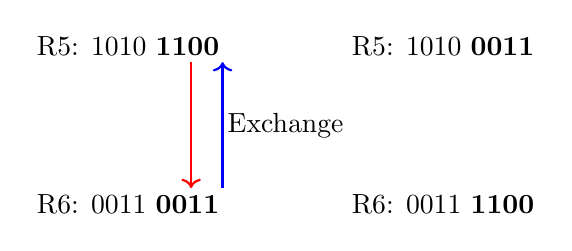
\begin{tikzpicture}
    % Visual representation
    \node (r5) at (0,2) {R5: 1010 \textbf{1100}};
    \node (r6) at (0,0) {R6: 0011 \textbf{0011}};
    
    \draw [->, thick, red] (0.8, 1.8) -- (0.8, 0.2);
    \draw [->, thick, blue] (1.2, 0.2) -- (1.2, 1.8);
    
    \node at (4,2) {R5: 1010 \textbf{0011}};
    \node at (4,0) {R6: 0011 \textbf{1100}};
    
    \node at (2,1) {Exchange};
\end{tikzpicture}
\end{center}
\end{solutionbox}
\begin{mnemonicbox}
``MAMS'' (Mask, And, Move, Swap)
\end{mnemonicbox}

\questionmarks{4}{b}{4}
\textbf{Write an 8051 Assembly Language Program to blink LED interfaced at port P1.0 at time interval of 1ms.}

\begin{solutionbox}
\textbf{Answer}:

\begin{lstlisting}[language={[x86masm]Assembler}]
      ORG 0000H        ; Start at memory location 0000H
MAIN: CPL P1.0         ; Complement P1.0 (toggle LED)
      ACALL DELAY      ; Call delay subroutine
      SJMP MAIN        ; Loop forever

DELAY: MOV R7, #2      ; Load R7 for outer loop (2)
DELAY1: MOV R6, #250   ; Load R6 for inner loop (250)
DELAY2: NOP            ; No operation (consume time)
        NOP            ; Additional delay
        DJNZ R6, DELAY2 ; Decrement R6 & loop until zero
        DJNZ R7, DELAY1 ; Decrement R7 & loop until zero
        RET            ; Return from subroutine
\end{lstlisting}

\begin{center}
\begin{tikzpicture}[node distance=2cm, auto]
    \node [draw, circle] (start) {Start};
    \node [gtu block, below of=start] (toggle) {Toggle P1.0};
    \node [gtu block, below of=toggle] (delay) {Delay 1ms};
    
    \draw [gtu arrow] (start) -- (toggle);
    \draw [gtu arrow] (toggle) -- (delay);
    \draw [gtu arrow] (delay) -- ++(2,0) |- (toggle);
\end{tikzpicture}
\end{center}
\end{solutionbox}
\begin{mnemonicbox}
``TCDL'' (Toggle, Call, Delay, Loop)
\end{mnemonicbox}

\questionmarks{4}{c}{7}
\textbf{List Addressing Modes of 8051 Microcontroller and explain them with at least one example.}

\begin{solutionbox}
\textbf{Answer}:

\begin{center}
\captionof{table}{8051 Addressing Modes}
\begin{tabular}{|l|l|l|}
\hline
\textbf{Addressing Mode} & \textbf{Description} & \textbf{Example} \\ \hline
\textbf{Register} & Uses registers (R0-R7) & \code{MOV A, R0} (Move R0 to A) \\ \hline
\textbf{Direct} & Uses direct memory address & \code{MOV A, 30H} (Move data from 30H to A) \\ \hline
\textbf{Register Indirect} & Uses register as pointer & \code{MOV A, @R0} (Move data from address in R0 to A) \\ \hline
\textbf{Immediate} & Uses constant data & \code{MOV A, \#25H} (Load A with 25H) \\ \hline
\textbf{Indexed} & Base address + offset & \code{MOVC A, @A+DPTR} (Code memory access) \\ \hline
\textbf{Bit} & Operates on individual bits & \code{SETB P1.0} (Set bit 0 of Port 1) \\ \hline
\textbf{Implied} & Implicit operand & \code{RRC A} (Rotate A right through carry) \\ \hline
\end{tabular}
\end{center}

\begin{center}
\begin{tikzpicture}[node distance=3cm]
    % Reg Direct Indir
    \node [gtu block] (reg) {Register\\MOV A, R5};
    \node [gtu block, right of=reg] (direct) {Direct\\MOV A, 40H};
    \node [gtu block, right of=direct] (indir) {Indirect\\MOV A, @R1};
    
    \node [below=0.2cm of reg, font=\tiny] {R5 $\to$ A};
    \node [below=0.2cm of direct, font=\tiny] {Mem[40H] $\to$ A};
    \node [below=0.2cm of indir, font=\tiny] {Mem[R1] $\to$ A};
\end{tikzpicture}
\end{center}
\end{solutionbox}
\begin{mnemonicbox}
``RIDDIBM'' (Register, Immediate, Direct, Data, Indirect, Bit, iMplied)
\end{mnemonicbox}

\orquestionmarks{4}{a}{3}
\textbf{Write an 8051 Assembly Language Program to add the byte in register R2 and R3, put the result in external RAM 2040h (LSB) and 2041h (MSB).}

\begin{solutionbox}
\textbf{Answer}:

\begin{lstlisting}[language={[x86masm]Assembler}]
      MOV A, R2      ; Move R2 to accumulator
      ADD A, R3      ; Add R3 to accumulator
      MOV DPTR, #2040H ; Set DPTR to external RAM address 2040H
      MOVX @DPTR, A  ; Store the result (LSB) at 2040H
      
      MOV A, #00H    ; Clear accumulator
      ADDC A, #00H   ; Add carry flag to accumulator
      INC DPTR       ; Increment DPTR to 2041H
      MOVX @DPTR, A  ; Store the result (MSB) at 2041H
\end{lstlisting}

\begin{itemize}
    \item Uses \code{MOVX} for external RAM access
    \item Uses \code{ADDC} to handle potential carry (result > 255)
\end{itemize}
\end{solutionbox}
\begin{mnemonicbox}
``MASIM'' (Move, Add, Store, Increment, Move again)
\end{mnemonicbox}

\orquestionmarks{4}{b}{4}
\textbf{For 8051 Microcontroller with a crystal frequency of 12 MHz, generate a delay of 5ms.}

\begin{solutionbox}
\textbf{Answer}:

\begin{lstlisting}[language={[x86masm]Assembler}]
      ; Delay of 5ms with 12MHz Crystal (1 machine cycle = 1 microsec)
DELAY: MOV R7, #5     ; 5 loops of 1ms each
LOOP1: MOV R6, #250   ; 250 x 4 microsec = 1000 microsec = 1ms
LOOP2: NOP            ; 1 microsec
       NOP            ; 1 microsec
       DJNZ R6, LOOP2 ; 2 microsec (if jump taken)
       DJNZ R7, LOOP1 ; Repeat 5 times for 5ms
       RET            ; Return from subroutine
\end{lstlisting}

\textbf{Calculation}:
\begin{itemize}
    \item 12MHz crystal = 1$\mu$s machine cycle
    \item Inner loop: 2 NOPs (2$\mu$s) + DJNZ (2$\mu$s) = 4$\mu$s per iteration
    \item 250 iterations $\times$ 4$\mu$s = 1000$\mu$s = 1ms
    \item Outer loop: 5 iterations $\times$ 1ms = 5ms
\end{itemize}
\end{solutionbox}
\begin{mnemonicbox}
``LOON-5'' (LOOp Nested for 5ms)
\end{mnemonicbox}

\orquestionmarks{4}{c}{7}
\textbf{Explain any seven Arithmetic Instructions with example for 8051 Microcontroller.}

\begin{solutionbox}
\textbf{Answer}:

\begin{center}
\captionof{table}{Arithmetic Instructions}
\begin{tabular}{|l|l|l|l|}
\hline
\textbf{Instruction} & \textbf{Function} & \textbf{Example} & \textbf{Flag Affected} \\ \hline
\textbf{ADD A,src} & Add source to A & \code{ADD A,R0} & C, OV, AC \\ \hline
\textbf{ADDC A,src} & Add source + carry to A & \code{ADDC A,\#25H} & C, OV, AC \\ \hline
\textbf{SUBB A,src} & Subtract source + borrow from A & \code{SUBB A,@R1} & C, OV, AC \\ \hline
\textbf{INC} & Increment by 1 & \code{INC R3} & None \\ \hline
\textbf{DEC} & Decrement by 1 & \code{DEC A} & None \\ \hline
\textbf{MUL AB} & Multiply A and B & \code{MUL AB} & C, OV \\ \hline
\textbf{DIV AB} & Divide A by B & \code{DIV AB} & C, OV \\ \hline
\end{tabular}
\end{center}
\end{solutionbox}
\begin{mnemonicbox}
``ACID-IBM'' (Add, Carry add, Inc, Dec, Mul, Borrow subtract, Divide)
\end{mnemonicbox}

\questionmarks{5}{a}{3}
\textbf{List Applications of microcontroller in various fields.}

\begin{solutionbox}
\textbf{Answer}:

\begin{center}
\captionof{table}{Microcontroller Applications}
\begin{tabular}{|l|l|}
\hline
\textbf{Field} & \textbf{Applications} \\ \hline
\textbf{Consumer Electronics} & TV, washing machine, microwave, remote control \\ \hline
\textbf{Automotive} & Engine control, anti-lock braking, airbag systems \\ \hline
\textbf{Industrial} & Automation, robotics, process control \\ \hline
\textbf{Medical} & Patient monitoring, medical instruments, implants \\ \hline
\textbf{Home Automation} & Smart lighting, security systems, HVAC control \\ \hline
\textbf{Communication} & Mobile phones, routers, modems \\ \hline
\textbf{Aerospace} & Navigation systems, flight control, satellite systems \\ \hline
\end{tabular}
\end{center}
\end{solutionbox}
\begin{mnemonicbox}
``CHAIM-MA'' (Consumer, Home, Automotive, Industrial, Medical, Mobile, Aerospace)
\end{mnemonicbox}

\questionmarks{5}{b}{4}
\textbf{Interface Relay with 8051 microcontroller.}

\begin{solutionbox}
\textbf{Answer}:

\begin{center}
\begin{circuitikz}
    \draw (0,0) node[gtu block, minimum height=3cm] (cpu) {8051\\P1.0};
    \draw (3,0) node[gtu block, minimum height=2cm] (driver) {Driver\\ULN2003};
    \draw (6,0) coordinate (coil);
    
    \draw [->] (cpu.east) -- (driver.west);
    \draw (driver.east) -- (coil) to[L, l=Relay] ++(0,2) node[vcc] {+12V};
    
    % Diode
    \draw (coil) ++(0.5,0) to[Do, l=1N4007] ++(0,2);
    
    \node [right] at (6.5, 1) {Protection Diode};
\end{circuitikz}
\end{center}

\textbf{Working}:
\begin{enumerate}
    \item 8051 sends control signal from P1.0
    \item Driver amplifies current to drive relay
    \item Protection diode prevents back EMF damage
    \item Relay switches connected devices
\end{enumerate}
\end{solutionbox}
\begin{mnemonicbox}
``DRIPS'' (Driver, Relay, Input from µC, Protection diode, Switching)
\end{mnemonicbox}

\questionmarks{5}{c}{7}
\textbf{Interface LCD with 8051 microcontroller.}

\begin{solutionbox}
\textbf{Answer}:

\begin{center}
\begin{circuitikz}
    % LCD Block
    \draw (4,0) rectangle (9,6);
    \node at (6.5, 5.5) {16x2 LCD};
    
    % 8051 Block
    \draw (-2,0) rectangle (1,6);
    \node at (-0.5, 5.5) {8051};
    
    % Data Lines
    \foreach \y [count=\i from 0] in {0.5, 1, 1.5, 2, 2.5, 3, 3.5, 4} {
        \draw (1, \y) -- (4, \y); 
        \node [left, font=\tiny] at (1,\y) {P2.\i};
        \node [right, font=\tiny] at (4,\y) {D\i};
    }
    \node at (2.5, 2) {Data Bus (8-bit)};
    
    % Control Lines
    \draw (1, 5) -- (4, 5); \node [left, font=\tiny] at (1,5) {P1.0}; \node [right, font=\tiny] at (4,5) {RS};
    \draw (1, 4.7) -- (4, 4.7); \node [left, font=\tiny] at (1,4.7) {P1.1}; \node [right, font=\tiny] at (4,4.7) {RW};
    \draw (1, 4.4) -- (4, 4.4); \node [left, font=\tiny] at (1,4.4) {P1.2}; \node [right, font=\tiny] at (4,4.4) {E};

    % Power Pot
    \draw (6.5, 0) -- ++(0,-1) node[ground]{};
    \node at (7.5, -0.5) {Pot for Contrast};
\end{circuitikz}
\end{center}

\textbf{Connections}:
\begin{itemize}
    \item \textbf{Control Lines}: RS (P1.0), RW (P1.1), E (P1.2)
    \item \textbf{Data Lines}: D0-D7 connected to Port 2
\end{itemize}

\textbf{Initialization Code}:
\begin{lstlisting}[language={[x86masm]Assembler}]
MOV A, #38H      ; 2 lines, 5x7 matrix
ACALL COMMAND
MOV A, #0EH      ; Display ON, cursor ON
ACALL COMMAND
MOV A, #01H      ; Clear LCD
ACALL COMMAND
MOV A, #06H      ; Increment cursor
ACALL COMMAND
\end{lstlisting}
\end{solutionbox}
\begin{mnemonicbox}
``CIDER-8'' (Control lines, Initialize, Data bus, Enable, Register select, 8-bit mode)
\end{mnemonicbox}

\orquestionmarks{5}{a}{3}
\textbf{Draw Interfacing of LED with 8051 microcontroller.}

\begin{solutionbox}
\textbf{Answer}:

\begin{center}
\begin{circuitikz}
    \draw (0,0) node[gtu block, minimum height=3cm] (cpu) {8051\\P1.0};
    
    \draw (cpu.east) -- ++(1,0) to[R, l=220$\Omega$] ++(2,0) to[leD, l=LED, invert] ++(0,1.5) node[vcc] {+5V};
\end{circuitikz}
\end{center}

\textbf{Working Principle}:
\begin{itemize}
    \item Active-Low configuration: LED ON when pin = 0
    \item Current limiting resistor (220$\Omega$) protects LED
    \item Max current approx 10-20mA
\end{itemize}
\end{solutionbox}
\begin{mnemonicbox}
``CIRCLE'' (Current limiting Resistor, IO pin, Cathode to LED, LED to Earth/ground)
\end{mnemonicbox}

\orquestionmarks{5}{b}{4}
\textbf{Interface DC Motor with 8051 microcontroller.}

\begin{solutionbox}
\textbf{Answer}:

\begin{center}
\begin{circuitikz}
    \node [gtu block, minimum height=2.5cm] (cpu) {8051};
    \node [gtu block, right of=cpu, node distance=4cm, minimum height=2.5cm] (driver) {L293D\\Driver};
    \node [right of=driver, node distance=3cm, circle, draw] (motor) {M};
    
    \draw [->] (cpu.east) ++(0,0.5) -- node[above] {P1.0} (driver.west |- 0,0.5);
    \draw [->] (cpu.east) ++(0,-0.5) -- node[below] {P1.1} (driver.west |- 0,-0.5);
    
    \draw (driver.east) ++(0,0.5) -- (motor.north);
    \draw (driver.east) ++(0,-0.5) -- (motor.south);
    
    \node [above of=driver] {+12V (Motor Supply)};
\end{circuitikz}
\end{center}

\begin{center}
\captionof{table}{Motor Control Logic}
\begin{tabular}{|l|l|l|}
\hline
\textbf{P1.0} & \textbf{P1.1} & \textbf{Motor Action} \\ \hline
0 & 0 & Stop (Brake) \\ \hline
0 & 1 & Clockwise \\ \hline
1 & 0 & Counter-clockwise \\ \hline
1 & 1 & Stop (Free-running) \\ \hline
\end{tabular}
\end{center}
\end{solutionbox}
\begin{mnemonicbox}
``DICER'' (Driver chip, Input from µC, Control logic, Enable motor, Rotation)
\end{mnemonicbox}

\orquestionmarks{5}{c}{7}
\textbf{Interface DAC0808 with 8051 microcontroller.}

\begin{solutionbox}
\textbf{Answer}:

\begin{center}
\begin{circuitikz}
    \node [gtu block, minimum height=2.5cm] (cpu) {8051\\Port 1};
    \node [gtu block, right of=cpu, node distance=4cm, minimum height=2.5cm] (dac) {DAC0808};
    \node [gtu block, right of=dac, node distance=3cm] (opamp) {Op-Amp\\I to V};
    
    \draw [->] (cpu) -- node [above] {8-bit Data} (dac);
    \draw [->] (dac) -- node [above] {Current} (opamp);
    \draw [->] (opamp.east) -- ++(1,0) node [right] {Analog $V_{out}$};
    
    \node [below of=dac] {Ref Voltage, GND, -VEE};
\end{circuitikz}
\end{center}

\textbf{Connections}:
\begin{itemize}
    \item P1.0-P1.7 $\to$ D0-D7 inputs of DAC
    \item DAC output is current, converted to voltage by Op-Amp
\end{itemize}

\textbf{Applications}: Waveform generation, Motor speed control
\end{solutionbox}
\begin{mnemonicbox}
``DACR'' (Digital input, Analog output, Conversion, Reference voltage)
\end{mnemonicbox}

\end{document}
